\subsection*{Экспериментальная установка}

Кванты, испытавшие комптоновское рассеяние в мишени, регистрируются сцинтилляционным счетчиком. Счетчик состоит из фотоэлектронного умножителя 3 (далее ФЭУ) и сцинтиллятора $4$. Сцинтиллятором служит кристалл NaI(Tl) цилиндрической формы диаметром 40 мм и высотой 40 мм, его выходное окно находится в оптическом контакте с фотокатодом ФЭУ. Сигналы, возникающие на аноде ФЭУ, подаются на ЭВМ для амплитудного анализа. Кристалл и ФЭУ расположены в светонепроницаемом блоке, укрепленном на горизонтальной штанге. 

\begin{figure}[h]
    \centering
    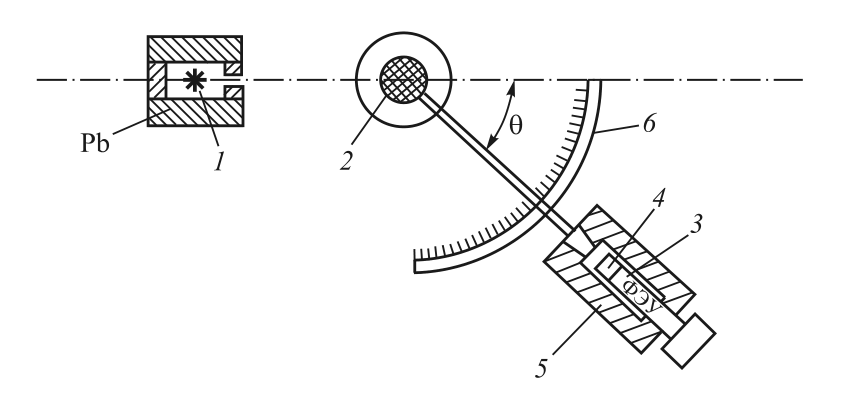
\includegraphics[width=0.45\textwidth]{figures/exp.png}
    \caption{Блок схема устаноки по рассеянию $\gamma$-квантов}
    \label{fig:exp}
\end{figure}

Штанга вместе с этим блоком может вращаться относительно мишени, угол поворота $\theta$ отсчитывается по лимбу $6$. 
Погрешность измерения угла поворота оценим в $2^{\circ}$, и выберем сдвиг на постоянный угол, как независимый параметр.
